\chapter{Datasets}
\label{cha:datasets}

In the previous chapter, we presented the fundamentals of highly overlapped signals.
To study these signals, suitable and controlled data is of paramount importance since many methods rely on audio datasets for development and evaluation.
Often, suitable audio material is not publicly available which is why we created our own data.
In the following sections, we present three data sets which we helped creating with the aim to fill this gap and which will be used in subsequent experiments.

\section{Unison Mixtures}
\label{sec:unison_dataset}

\marginpar{This subsection is based on~\cite{stoeter14} where the scenario of unsion mixtures was first introduced.}

Synthetic mixtures are created from single source sounds, e.g., through (often random) summation. 
In speech, it is common to mix clean speech and noise~\cite{varga93} or different clean speech signals such as~\cite{garofolo93} to generate mixtures.
By contrast, the conversational aspect of human-to-human communication is lost.
Compared to speech, musical content usually does share familiar orchestration and can hardly be superimposed randomly, and the summing of isolated random notes from musical instrument databases does not reflect musical performances.
On the positive side, there are use-cases for single note datasets such as for evaluation of \(F0\) estimation algorithms or the detection of instruments.
Furthermore, single note datasets allow to use the data to synthesize musical score as long as the recordings have enough variance of expressions.
It also allows to quickly generate a large amount of mixtures using randomly permuted mixtures, fostering applications in machine learning.

As an exception compared to other music scenarios, when all instruments play~\emph{in unison}, single note datasets are appropriate to approximate real mixtures:

\begin{itemize}
  \item A random summation of multiple instruments playing the same note does not necessarily differ from realistic unison mixture.
  \item When notes are played with vibrato, having access to the individual modulation patterns can help to study the influence of modulations in a systematic fashion.
  \item Unison mixtures are part of many classical compositions, to extend the timbre of a note.
\end{itemize}

\par
In order to create a dataset, we could use existing single note datasets such as the \emph{Univ. of Iowa Musical Instrument Sample Database}\footnote{\url{http://theremin.music.uiowa.edu/index.htm}}, created from acoustic recording sessions.
However, to better study the influence of vibrato we require extended control over certain parameters such as: note duration, vibrato duration, exact fundamental frequency, vibrato rate, vibrato extend, reproducibility, loudness or expression.
\par
Also, it is important to note that vibrato techniques differ between instruments: whereas the English horn and the flute only produce a very subtle modulation, the violin and tenor sax are capable of powerful frequency modulations~\cite{gilbert05}.
\par
We therefore generated the notes using a software sampler \textsc{Vienna Symphonic Library}\footnote{\url{https://vsl.co.at}} which allows us to control the parameters such as the vibrato.
All our test stimuli have a duration of three seconds.
Items were equalized in loudness by using an iterative calculation of the loudness algorithm of the time varying Zwicker model~\cite{zwicker13}. 
We used an implementation released in~\cite{genesis12}. 
\par
We rendered 29 notes of C4, resulting in 841 unique unison instrument mixtures per pitch class.
An except of the instruments is listed in Table~\ref{tab:testset}.
The dataset is available from~\cite{oss_unison}.

\begin{table}
\begin{center}
\footnotesize
\begin{tabular}{ l l l}
  Instrument & Vibrato &  General MIDI \# \\
  \hline
  Violin & yes & 40 \\
  Viola & yes & 41 \\
  Violon Cello & yes & 42 \\
  Trumpet & no & 56 \\
  Trombone & no & 57\\
  Horn & no & 60  \\
  Bariton Sax & yes & 67 \\
  Oboe & no & 68\\
  Clarinet & no & 71\\
  Flute & yes & 73\\
\end{tabular}
\end{center}
\caption{Selected Instruments from the \emph{Unison Source Separation Dataset}~\cite{oss_unison})as used in~\cite{stoeter14, stoeter16}.}
\label{tab:testset}
\end{table}

To evaluate the level of overlap, we created a small experiment where we computed the average W-disjoint orthogonality \(WDO\) metric for 1000 random combinations of mixtures for different separation scenarios.
It turned out that for speech separation of \(k=2\) speakers, (\(WDO=0.9\)) and for the vocal accompaniment scenario (\(WDO=0.87\)), surprisingly similar even though both scenarios are so fundamentally different.
In the case of two instruments playing in unison the average WDO is \(0.65\), indicating that a good separation in the time frequency domain is more challenging, thus making the dataset a useful addition compared to existing scenarios.

% \begin{figure}
% \begin{tikzpicture}
% 	\begin{axis}[
% 		xlabel=Number of Sources,
%     ylabel=Separability/WDO]
%     % speakers
% 	\addplot[color=red,mark=x] coordinates {
% 		(2,0.9)
% 		(3,0.79)
% 		(4,0.69)
% 		(5,0.6)
% 		(6,0.536)
% 		(7,0.462)
% 		(8,0.4197)
% 		(9,0.352199)
% 		(10,0.32)
%   };
%   % single note
%   	\addplot[color=blue,mark=x] coordinates {
% 		(2,0.928)
% 		(3,0.864)
% 		(4,0.8)
% 		(5,0.77)
% 		(6,0.682)
% 		(7,0.637)
% 		(8,0.592)
% 		(9,0.5647)
% 		(10,0.5434)
%   };
%   % unison
%     \addplot[color=yellow,mark=x] coordinates {
% 		(2,0.626)
% 		(3,0.32)
% 		(4,0.2)
% 		(5,0.13)
% 		(6,0.083)
% 		(7,0.038)
% 		(8,0.025)
% 		(9,0.017)
% 		(10,0.01)
% 	};
% 	\end{axis}
% \end{tikzpicture}
% \end{figure}

\section{High Resolution Vibrato}

\marginpar{This subsection is based on the work that has been published in~\cite{stoeter15acm} together with my former student Michael Müller who helped with the experiments.}

Fundamental frequency \(F0\) estimation of a signal is a common task in audio signal processing with many applications. 
If the $F0$ varies over time, the complexity increases, and it is also more difficult to provide ground truth data for evaluation.

\begin{figure}[h]
  \centering
  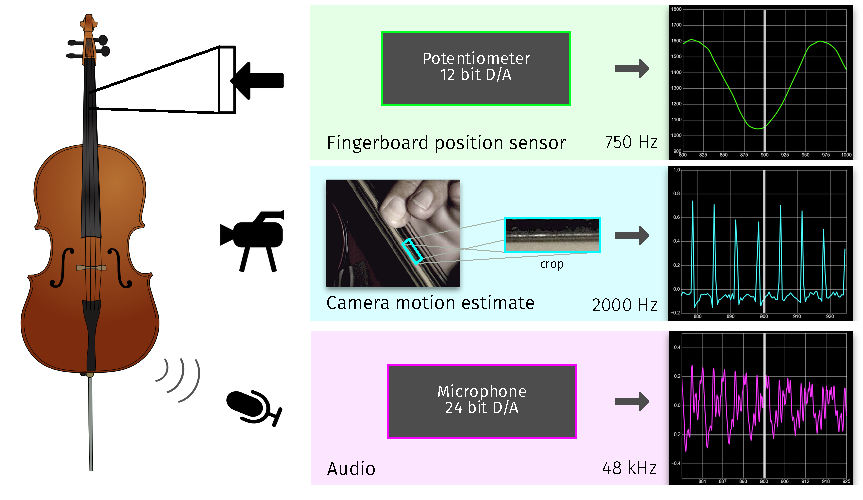
\includegraphics[width=\textwidth]{Chapters/04_Data/figures/teaser.pdf}
  \caption{Overview of the multi-modal data recorded for the proposed dataset.}
\label{fig:teaser_hdf0}
\end{figure}

% from 
For speech signals, an EGG device (also known as laryngograph) captures the excitation of the human vocal tract. 
This signal is then processed by an $F0$ estimator to generate the ground truth. 
Such a method is accepted in published research because the EGG signal is considered to be easier to process than speech. 
The retrieved F0-trajectory based on the EGG signal is easier to process and the generated annotations are considered as a good ground truth~\cite{pirker11, babacan13}.
Motivated by this, we propose a new data set for musical instruments where we recorded a violin cello with extra sensors on the fretboard in addition to audio and video.
We made use of multiple sensors to capture the most relevant processes involved in creating time-varying output signals as depicted in Figure~\ref{fig:teaser_hdf0}.
We included sensor recordings capturing the finger position on the fingerboard which is converted into an instantaneous frequency estimate.
We also included high speed video camera data to capture excitations from the string at 2000 fps.
Recording video data was inspired by the work of Davis et.\ al.\ in~\cite{Davis2014VisualMic} presenting a ``visual microphone'' which is able to observe sound solely with a camera, pointing to objects in the sound field. 
\par
In the proposed test set we chose the violin cello for the following reasons: (1) vibrato is used as a common style for expression, (2) there is an observable physical relationship between frequency modulation and vibrato, and (3) the instrument is large enough to embed sensors to capture the vibrato. The properties of the cello are studied by research in acoustics~\cite{woodhouse04, woodhouse99}.
\par
To capture major aspects of the cello while being played by a musician, we focus on three main observations: (1) Excitation caused by the moving bow; (2) the vibrating string, and (3) the finger, controlling the string length by rolling it on the fingerboard.
The main focus of the recordings is to analyze vibrato playing style. Since it is common that vibrato characteristics differ from musician to musician, all recordings were performed by two musicians. One is a professional cellist with 30 years of experience in a symphonic orchestra\footnote{\url{http://www.bambergerstreichquartett.de/de/Das_Quartett/Karlheinz_Busch}}.
The other recording was done by the author of this thesis, who has less than 1 hour per week of practice.
\par
Due to the width of fingerboard sensors and the attached cables we were able to equip two strings (G and A) allowing to record pitches ${G2, D3, D^\sharp3, E3, A3, B3, C4, C^\sharp4}$ from both musicians (see middle part of Figure~\ref{fig:teaser_hdf0}).
\par
The dataset includes time synchronous fingerboard positions and high-speed camera recordings. 
The derived motion estimates shows similarity to the EGG signals used in speech. 
The slowest feature rate of the set is 750 Hz, which enables to evaluate $F0$ estimators with high temporal resolution. 
\par
In~\cite{stoeter15acm}, we also showed how to derive high resolution $F0$ contours from the data which can be used to improve $F0$ estimators or help to analyze playing styles in recordings, usually relying on conventional $F0$ estimators based on the audio signal~\cite{mellody2000time}. 
By using sensor data samples from our test set, researchers get more robust and detailed data to compute features like mean vibrato frequency. 
Further, it can be used for synthesizers to add a natural vibrato by using the sensor data as modulation source.
\par
The resulting test set yields in $148$ recorded notes after removal of some notes due to errors in the sensor recordings.
By making this dataset public domain~\cite{oss_muserc} and including the raw recordings, we believe other researchers can benefit from the data and possibly generate their own derived data.

\section{Multitrack Data}

\marginpar{This subsection is based on parts of the work that has been published in~\cite{liutkus17, rafii}. The parts that are cited here were co-authored by me.}

Multitrack datasets are helpful, and often necessary to develop and evaluate methods on complex acoustic tasks such as source separation.
The Signal Separation Evaluation Campaign (SiSEC) is a solid indicator of the progress in research within the field of source separation \cite{sisec13, ono15, liutkus17, stoeter18sisec}.
% zafar begin
Building a good data-driven method for source separation relies heavily on a training dataset to learn the separation model. 
For professionally-produced or recorded music, the separated sources are often either unavailable or private. 
Indeed, they are considered amongst the most precious assets of right holders, and it is challenging to find isolated vocals and accompaniment of professional bands that are freely available for the research community to work on without copyright infringements.
% zafar end
In this context, the development of datasets for music separation was a long process. 
In early times, it was common for researchers to test their methods on private data. 
To the best of our knowledge, the first attempt at releasing a public dataset for evaluating vocals and accompaniment separation was the Music Audio Signal Separation (MASS) dataset~\cite{MTGMASSdb}.
It strongly boosted research in the area, even if it only featured 2.5 minutes of data. The breakthrough was made possible by some artists which made their mixed-down audio, as well as its constitutive stems (unmixed tracks), available under open licenses such as Creative Commons, or authorized scientists to use their material for research.
% 
The MASS dataset formed the core content of the early Signal Separation Evaluation Campaigns (SiSEC) \cite{vincent09}. 
For a long time, vocals separation methods were very demanding computationally and it was already considered extremely challenging to separate excerpts of only a few seconds.

In the following years, new datasets were proposed that improved over the MASS dataset in many directions. 
We briefly describe the most relevant ones below:

\begin{itemize}[leftmargin=*]
	\item The QUASI dataset was proposed to study the impact of different mixing scenarios on the separation quality. It  consists of the same tracks as in the MASS dataset, but kept full length and mixed by professional sound engineers.
	\item The MIR-1K~\cite{hsu10} and iKala~\cite{chan15} datasets were the first attempts to scale vocals separation up. They feature a higher number of samples (1000) than the previously available datasets. However, they consist of mono signals of very short and amateur karaoke recordings.
	\item The ccMixter~\cite{liutkus142} dataset was proposed as the first dataset to feature many full-length stereo tracks. Each one comes with a vocals and an accompaniment source. Although it is stereo, it often suffers from simplistic mixing of sources, making it unrealistic in some aspects.
	\item MedleyDB~\cite{bittner14} has been developed as a dataset to serve many purposes in music information retrieval. It consists of more than 100 full-length recordings, with all their constitutive sources. It is the first dataset to provide such a large amount of data to be used for audio separation research (more than 7 hours). Among all the material present in that dataset, 63 tracks feature singing voice.
	\item DSD100~\cite{liutkus17} was presented for SiSEC 2016. It features 100 full-length tracks originating from the 'Mixing Secret' Free Multitrack Download Library\footnote{\url{http://www.cambridge-mt.com/ms-mtk.htm}} of the Cambridge Music Technology, which is freely usable for research and educational purposes.
	The dataset consists of four predefined categories: \emph{bass, drums, vocals, and other}. An extended version, merging MedleyDB and DSD100 was recently released as MUSDB18~\cite{rafii17, stoeter18sisec}
\end{itemize}

Over the years, DSD100/MUSDB18 became one of the most used datasets for source separation. 
The dataset is still tiny in comparison to recent machine learning sets, but it proved to be large enough to help DNN-based methods to reach break through results in source separation~\cite{stoeter18sisec}.
\par
Working with multitrack audio files can be cumbersome due to its hierarchical structure that needs to be parsed.
Additionally, an accompanying software toolbox was developed in Python that permits the straightforward processing of the DSD100 dataset. This software is open source and was publicly broadcasted so as to allow the participants to run the evaluation themselves\footnote{\url{github.com/faroit/dsdtools}}.
\par
This package integrates with existing Python code, thus makes it easy to participate in the SISEC MUS tasks. The core of this package is calling a user-provided function that separates the mixtures from the DSD into several estimated target sources.

% \begin{code}
% \captionof{listing}{Full working code example to parse the full DSD100~\cite{liutkus17} dataset as \emph{NumPy} arrays and write out estimates (here: the mixture) into a predefined estimates directory.}
% \begin{minted}{python}
% import dsdtools

% def my_function(track):
%     estimates = {
%         'vocals': track.audio,
%         'accompaniment': track.audio,
%     }
%     return estimates

% dsd = dsdtools.DB(root_dir="./Volumes/Data/dsdtools")
% dsd.run(my_function, estimates_dir="path/to/estimates")
% \end{minted}
% \label{code:c-code}
% \end{code}

All details of this accompanying software tools may be found on its dedicated website\footnote{\url{https://sigsep.github.io}}.